%!TEX TS-program = lualatex
%!TEX encoding = UTF-8 Unicode

\documentclass[12pt, addpoints]{exam}

%\printanswers

\usepackage{graphicx}
	\graphicspath{{/Users/goby/Pictures/teach/163/lab/}
	{img/}} % set of paths to search for images

\usepackage{geometry}
\geometry{letterpaper, left=1.5in, bottom=1in}                   
%\geometry{landscape}                % Activate for for rotated page geometry
\usepackage[parfill]{parskip}    % Activate to begin paragraphs with an empty line rather than an indent
\usepackage{amssymb, amsmath}
\usepackage{mathtools}
	\everymath{\displaystyle}

\usepackage{fontspec}
\setmainfont[Ligatures={TeX}, BoldFont={* Bold}, ItalicFont={* Italic}, BoldItalicFont={* BoldItalic}, Numbers={OldStyle}]{Linux Libertine O}
\setsansfont[Scale=MatchLowercase,Ligatures=TeX]{Linux Biolinum O}
\setmonofont[Scale=MatchLowercase]{Linux Libertine Mono O}
\newfontfamily\liningnum[Numbers=Lining]{Linux Libertine O}
\usepackage{microtype}

\usepackage{pdflscape}

\usepackage{tikz}
\usetikzlibrary{trees}

\usepackage{forest}

% To define fonts for particular uses within a document. For example, 
% This sets the Libertine font to use tabular number format for tables.
 %\newfontfamily{\tablenumbers}[Numbers={Monospaced}]{Linux Libertine O}
% \newfontfamily{\libertinedisplay}{Linux Libertine Display O}

\usepackage{booktabs}
\usepackage{multicol}

\usepackage{caption}
	\captionsetup{labelsep=period, justification=raggedright} % Removes colon following figure / table number.
	\captionsetup{singlelinecheck=off}
	\captionsetup[table]{skip=0pt}

%\usepackage{tikz}
\tikzstyle{block} = [rectangle, draw, fill=white, rounded corners,
                 minimum size=2em]
\tikzstyle{branch} = [thick, draw]

\usetikzlibrary{positioning, backgrounds}

\tikzset{
	timeline/.style={text centered, text width=2cm},
	no edge from this parent/.style={
		every child/.append style={
			edge from parent/.style={draw=none}}},
}

\forestset{
	every leaf node/.style={
		if n children=0{#1}{}
	},
	every tree node/.style={
		if n children=0{}{#1}
	},
	mytree/.style={
		for tree={
			edge path={
				\noexpand\path [draw, thick, \forestoption{edge}] (!u.parent anchor) |- (.child anchor)\forestoption{edge label};
			},
			every tree node={draw=none,inner sep=0, outer sep=0, minimum size=0},
			every leaf node/.style={align=left},
			grow'=0,
			parent anchor=east, 
			child anchor=west,
			anchor=west,
			l sep=0.5cm,
			s sep=3mm,
			draw=none,
			if n children=0{tier=word}{}
		}
	}
}

\forestset{
	every leaf node/.style={
		if n children=0{#1}{}
	},
	every tree node/.style={
		if n children=0{}{#1}
	},
	Vtree/.style={
		for tree={
			edge path={
				\noexpand\path [draw, thick, \forestoption{edge}] (!u.parent anchor) -< (.child anchor)\forestoption{edge label};
			},
			every tree node={draw=none,inner sep=0, outer sep=0, minimum size=0},
			every leaf node/.style={align=left},
			grow'=0,
			parent anchor=east, 
			child anchor=west,
			anchor=west,
			l sep=0.5cm,
			s sep=3mm,
			draw=none,
			if n children=0{tier=word}{}
		}
	}
}

\usepackage{longtable}
%\usepackage{siunitx}
\usepackage{array}
\newcolumntype{L}[1]{>{\raggedright\let\newline\\\arraybackslash\hspace{0pt}}p{#1}}
\newcolumntype{C}[1]{>{\centering\let\newline\\\arraybackslash\hspace{0pt}}p{#1}}
\newcolumntype{R}[1]{>{\raggedleft\let\newline\\\arraybackslash\hspace{0pt}}p{#1}}

\usepackage{enumitem}
\setlist{leftmargin=*}
\setlist[1]{labelindent=\parindent}
\setlist[enumerate]{label=\textsc{\alph*}.}


\usepackage[sc]{titlesec}

%% Commands for Exam class
\renewcommand{\solutiontitle}{\noindent}
\unframedsolutions
\SolutionEmphasis{\bfseries}

\renewcommand{\questionshook}{%
	\setlength{\leftmargin}{-\leftskip}%
}

%Change \half command from 1/2 to .5
\renewcommand*\half{.5}

\pagestyle{headandfoot}
\firstpageheader{\textsc{bi}\,063 Evolution and Ecology}{}{\ifprintanswers\textbf{KEY}\else Name: \enspace \makebox[2.5in]{\hrulefill}\fi}
\runningheader{}{}{\footnotesize{pg. \thepage}}
\footer{}{}{}
\runningheadrule

\newcommand*\AnswerBox[2]{%
    \parbox[t][#1]{0.92\textwidth}{%
    \begin{solution}#2\end{solution}}
%    \vspace*{\stretch{1}}
}

\newenvironment{AnswerPage}[1]
    {\begin{minipage}[t][#1]{0.92\textwidth}%
    \begin{solution}}
    {\end{solution}\end{minipage}
    \vspace*{\stretch{1}}}

\newlength{\basespace}
\setlength{\basespace}{5\baselineskip}

%% To hide and show points
\newcommand{\hidepoints}{%
	\pointsinmargin\pointformat{}
}

\newcommand{\showpoints}{%
	\nopointsinmargin\pointformat{(\thepoints)}
}

\newcommand{\bumppoints}[1]{%
	\addtocounter{numpoints}{#1}
}


\begin{document}

\subsection*{Character similarities and phylogenetic trees}

Here are the results you should have for the presence/absence data set.

{\liningnum
\begin{longtable}[c]{@{}cC{0.32in}C{0.32in}C{0.32in}C{0.32in}C{0.32in}C{0.32in}@{}}
\toprule
Species & C1 & C2 & C3 & C4 & C5 & C6\tabularnewline
\midrule
	&	&	&	&	&	\tabularnewline
B	&
	1	& 
	1	& 
	0	&
	1	&
	1	&
	0	\tabularnewline[0.15in]
%
Y	& 
	1	&
	1	&
	0	&
	1	&
	1	&
	0	\tabularnewline[0.15in]
%
C	&
	0	&
	1	&
	0	&
	1	& 
	1	&
	0	\tabularnewline[0.15in]
%
F	&
	0	&
	0	&
	1	&
	1	&
	1	&
	0	\tabularnewline[0.15in]
%
A	&	
	0	&
	0	&
	1	&
	1	&
	1	&
	0	\tabularnewline[0.15in]
%
R	&
	0	&
	0	&
	0	&
	0	&
	1	&
	1	\tabularnewline[0.15in]
\bottomrule
\end{longtable}
}



%\question[2]
%Which species are the most similar? Why?

%\AnswerBox{5\baselineskip}{%
% B and Y, and F and A. Both pairs differ by only two nucleotides, the fewest number of all pairs.
%}

Careful inspection of the results will show you which species are most closely related. Notice that the blue-throated (\textsc{b}) and yellow-throated ({\textsc{y}) garblers share the most characters (4), suggesting they are most closely related among the species shown. In contrast, the red-footed chump (\textsc{r}) is most distantly related, sharing only one character with the other species. Recall from the previous handout that characters that are not shared are not useful for making phylogenetic trees. Therefore, ignore character C{\liningnum 6} for the rest of this exercise.

You can construct a phylogenetic tree  based on shared characters, following the steps
below. Try this on a piece of paper as you read along; you will do it for
real later \emph{and possibly on an exam.} 

\begin{enumerate}%[leftmargin=*, label=\alph*.]

\item Which pair of species share a character not shared with other species? 
Put the letters of those species at the top of the
chart. Put a dot below and between them. Draw lines connecting the two species to the
dot. Do this for each pair of very closely related species.

\item What species is most similar to one pair from part \textsc{a}? Put its letter
at the top and put a dot below it between it and either of the pair of species from part \textsc{a}.
Draw lines connecting the third species to the dot below the pair.

\item Repeat step \textsc{b} for each group of species, working from most similar to
least similar.

\end{enumerate}

The next several pages will walk you through this process. Be sure you understand each step because you will do this on your own with different data.

\newpage

Set the diagram up like this. The tick marks on the \textsc{y}-axis are for reference only and are not necessary.

\begin{tikzpicture}[scale=0.8]

\draw (0,0) -- coordinate (y axis mid) (0,10);
    	%ticks
%\foreach \y/\label in {0/10, 2/8, 4/6, 6/4, 8/2, 10/0}
\foreach \y in {0, 2, 4, 6, 8, 10}
	\draw (1pt,\y) -- (-3pt,\y) 
		node[anchor=east] {}; %{\label};                  
                 
\foreach \x/\species in {0/C, 2/B,4/F, 6/R, 8/Y, 10/A}
	\node [block] at (15,\x) (\species) {\species} ;
                 
\end{tikzpicture}

Plot two of the most similar species, B and Y. They share character C{\liningnum 1}, which is not shared with other species. After you plot these, the diagram should look like this.

\begin{tikzpicture}[scale=0.8]

\draw (0,0) -- coordinate (y axis mid) (0,10);
    	%ticks
%\foreach \y/\label in {0/10, 2/8, 4/6, 6/4, 8/2, 10/0}
\foreach \y in {0, 2, 4, 6, 8, 10}
	\draw (1pt,\y) -- (-3pt,\y) 
		node[anchor=east] {};% {\label};                  

\node [block] at (2,10.5) (b) {B};
\node [block] at (4,10.5) (y) {Y};
\path[branch] (b.south) -- (3,8);
\path[branch] (y.south) -- (3,8);
                 
\foreach \x/\species in {0/C, 4/F, 6/R, 10/A}
	\node [block] at (15,\x)  {\species} ;
                 
\end{tikzpicture}

\newpage

Now add species C, which shares character C{\liningnum 2} with B and Y (and therefore next most similar).  It now looks like this.

\begin{tikzpicture}[scale=0.8]

\draw (0,0) -- coordinate (y axis mid) (0,10);
    	%ticks
%\foreach \y/\label in {0/10, 2/8, 4/6, 6/4, 8/2, 10/0}
\foreach \y in {0, 2, 4, 6, 8, 10}
	\draw (1pt,\y) -- (-3pt,\y) 
		node[anchor=east] {};% {\label};                  

\node [block] at (2,10.5) (b) {B};
\node [block] at (4,10.5) (y) {Y};
\node [block] at (6,10.5) (c) {C};

\node (by) at (3,8){};
\node (byc) at (5,6){};

\path [branch] (b.south) -- (by.center); 
\path [branch] (y.south) -- (by.center);
\path [branch] (c.south) -- (byc.center);
\path [branch] (by.center) -- (byc.center);
                 
\foreach \x/\species in {4/F, 6/R, 10/A}
	\node [block] at (15,\x)  {\species} ;
                 
\end{tikzpicture}

Species F and A share character C{\liningnum 4} with B, Y, and C but notice that F and A share character C{\liningnum 3} only with each other so connect them first like you did for B and Y.

\begin{tikzpicture}[scale=0.8]

\draw (0,0) -- coordinate (y axis mid) (0,10);
    	%ticks
%\foreach \y/\label in {0/10, 2/8, 4/6, 6/4, 8/2, 10/0}
\foreach \y in {0, 2, 4, 6, 8, 10}
	\draw (1pt,\y) -- (-3pt,\y) 
		node[anchor=east] {};% {\label};                  

\node [block] at (2,10.5) (b) {B};
\node [block] at (4,10.5) (y) {Y};
\node [block] at (6,10.5) (c) {C};
\node [block] at (8,10.5) (f) {F};
\node [block] at (10,10.5) (a) {A};

\node (by) at (3,8){};
\node (byc) at (5,6){};
\node (fa) at (9,8){};

\path [branch] (b.south) -- (by.center); 
\path [branch] (y.south) -- (by.center);
\path [branch] (c.south) -- (byc.center);
\path [branch] (by.center) -- (byc.center);
\path [branch] (f.south) -- (fa.center);
\path [branch] (a.south) -- (fa.center);
                 
\foreach \x/\species in {6/R}
	\node [block] at (15,\x)  {\species} ;
                 
\end{tikzpicture}

\newpage

Now connect the F and A pair to B, Y, and C because they all share character C{\liningnum 4}.  It looks like this.

\begin{tikzpicture}[scale=0.8]

\draw (0,0) -- coordinate (y axis mid) (0,10);
    	%ticks
%\foreach \y/\label in {0/10, 2/8, 4/6, 6/4, 8/2, 10/0}
\foreach \y in {0, 2, 4, 6, 8, 10}
	\draw (1pt,\y) -- (-3pt,\y) 
		node[anchor=east] {};% {\label};                  

\node [block] at (2,10.5) (b) {B};
\node [block] at (4,10.5) (y) {Y};
\node [block] at (6,10.5) (c) {C};
\node [block] at (8,10.5) (f) {F};
\node [block] at (10,10.5) (a) {A};

\node (by) at (3,8){};
\node (byc) at (5,6){};
\node (fa) at (9,8){};
\node (bycfa) at (7,4){};

\path [branch] (b.south) -- (by.center); 
\path [branch] (y.south) -- (by.center);
\path [branch] (c.south) -- (byc.center);
\path [branch] (by.center) -- (byc.center);
\path [branch] (f.south) -- (fa.center);
\path [branch] (a.south) -- (fa.center);
\path [branch] (fa.center) -- (bycfa.center);
\path [branch] (byc.center) -- (bycfa.center);

\foreach \x/\species in {6/R}
	\node [block] at (15,\x)  {\species} ;
                 
\end{tikzpicture}

Finally, connect species R to the rest. It shares only character C{\liningnum 5} with the other five species.

\begin{tikzpicture}[scale=0.8]

\draw (0,0) -- coordinate (y axis mid) (0,10);
    	%ticks
%\foreach \y/\label in {0/10, 2/8, 4/6, 6/4, 8/2, 10/0}
\foreach \y in {0, 2, 4, 6, 8, 10}
	\draw (1pt,\y) -- (-3pt,\y) 
		node[anchor=east] {};% {\label};                  

\node [block] at (2,10.5) (b) {B};
\node [block] at (4,10.5) (y) {Y};
\node [block] at (6,10.5) (c) {C};
\node [block] at (8,10.5) (f) {F};
\node [block] at (10,10.5) (a) {A};
\node [block] at (12,10.5) (r) {R};

\node (by) at (3,8){};
\node (byc) at (5,6){};
\node (fa) at (9,8){};
\node (bycfa) at (7,4){};
\node (all) at (11,0){};

\path [branch] (b.south) -- (by.center); 
\path [branch] (y.south) -- (by.center);
\path [branch] (c.south) -- (byc.center);
\path [branch] (by.center) -- (byc.center);
\path [branch] (f.south) -- (fa.center);
\path [branch] (a.south) -- (fa.center);
\path [branch] (fa.center) -- (bycfa.center);
\path [branch] (byc.center) -- (bycfa.center);
\path [branch] (bycfa.center) -- (all.center);
\path [branch] (r.south) -- (all.center);

\end{tikzpicture}

\newpage

You can draw short marks across some of the lines, labeled with the character numbers, to show which characters are shared among the different species.

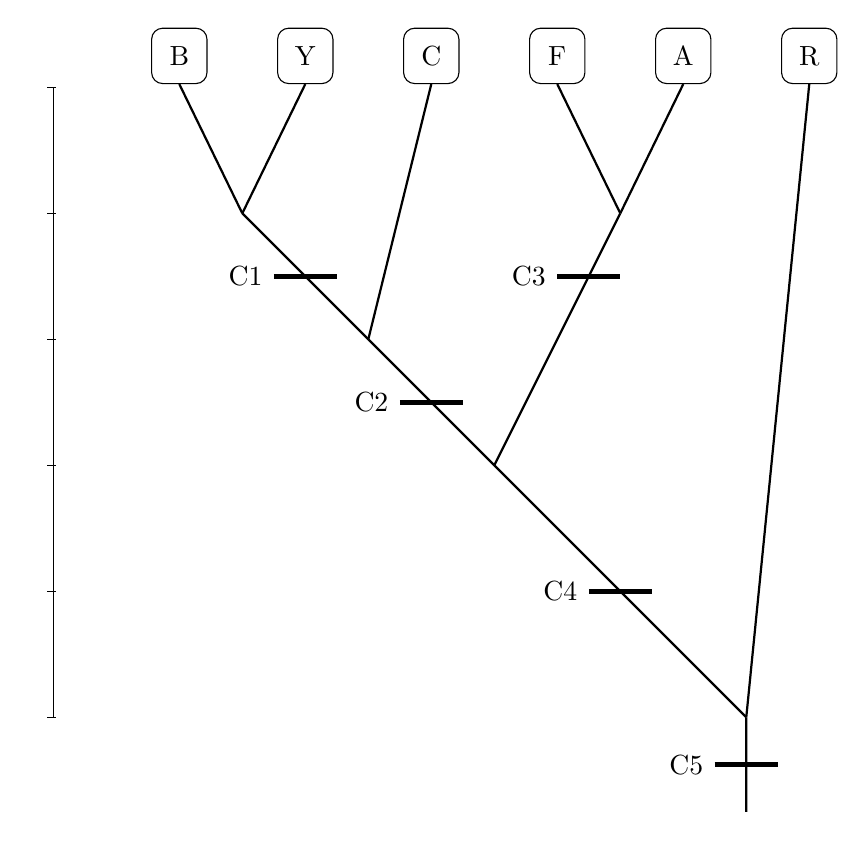
\begin{tikzpicture}[scale=0.8]

\draw (0,0) -- coordinate (y axis mid) (0,10);
    	%ticks
%\foreach \y/\label in {0/10, 2/8, 4/6, 6/4, 8/2, 10/0}
\foreach \y in {0, 2, 4, 6, 8, 10}
	\draw (1pt,\y) -- (-3pt,\y) 
		node[anchor=east] {};% {\label};                  

\node [block] at (2,10.5) (b) {B};
\node [block] at (4,10.5) (y) {Y};
\node [block] at (6,10.5) (c) {C};
\node [block] at (8,10.5) (f) {F};
\node [block] at (10,10.5) (a) {A};
\node [block] at (12,10.5) (r) {R};

\node (by) at (3,8){};
\node (byc) at (5,6){};
\node (fa) at (9,8){};
\node (bycfa) at (7,4){};
\node (all) at (11,0){};

\path [branch] (b.south) -- (by.center); 
\path [branch] (y.south) -- (by.center);
\path [branch] (c.south) -- (byc.center);
\path [branch] (by.center) -- (byc.center);
\path [branch] (f.south) -- (fa.center);
\path [branch] (a.south) -- (fa.center);
\path [branch] (fa.center) -- (bycfa.center);
\path [branch] (byc.center) -- (bycfa.center);
\path [branch] (bycfa.center) -- (all.center);
\path [branch] (r.south) -- (all.center);
\path [branch] (all.center) -- (11,-1.5);

\draw [ultra thick] (3.5,7) node [left] {C\liningnum 1} to (4.5,7) ;
\draw [ultra thick] (5.5,5) node [left] {C\liningnum 2} to (6.5,5) ;
\draw [ultra thick] (8.5,2) node [left] {C\liningnum 4} to (9.5,2) ;
\draw [ultra thick] (8,7) node [left] {C\liningnum 3} to (9,7) ;
\draw [ultra thick] (10.5,-0.75) node [left] {C\liningnum 5} to (11.5,-0.75) ;

\end{tikzpicture}

Now you have a phylogenetic tree that shows the relationships among species based on shared characters.  If you want to know which characters are shared between, say, the blue-throated garbler (\textsc{b}) and the field twitterer (\textsc{f}),  just follow the lines down from both species until you come to the spot where they join.  Then look at the tick marks below that point. The blue-throated garbler and the field twitterer share characters C{\liningnum 4} (knows that the bird is a word) and C{\liningnum 5} (rocks in the tree tops all day long). 

Here are the results again. Compare them to the final tree above. Make a mark for character C{\liningnum 6} on the tree above. Notice that it cannot show relationships because it is found on in the red-footed chump (\textsc{r}).

{\liningnum
\begin{longtable}[c]{@{}cC{0.32in}C{0.32in}C{0.32in}C{0.32in}C{0.32in}C{0.32in}@{}}
\toprule
Species & C1 & C2 & C3 & C4 & C5 & C6\tabularnewline
\midrule
B	&
	1	& 
	1	& 
	0	&
	1	&
	1	&
	0	\tabularnewline
%
Y	& 
	1	&
	1	&
	0	&
	1	&
	1	&
	0	\tabularnewline
%
C	&
	0	&
	1	&
	0	&
	1	& 
	1	&
	0	\tabularnewline
%
F	&
	0	&
	0	&
	1	&
	1	&
	1	&
	0	\tabularnewline
%
A	&	
	0	&
	0	&
	1	&
	1	&
	1	&
	0	\tabularnewline
%
R	&
	0	&
	0	&
	0	&
	0	&
	1	&
	1	\tabularnewline
\bottomrule
\end{longtable}
}

\newpage

\thispagestyle{empty}

\begin{questions}
	
\begin{landscape}

Now, make phylogenetic trees from the following presence/absence data sets. Use a separate sheet of paper to draw your trees. Ask your instructor to check your trees to be sure each is correct. %your phylogenetic trees on.

\liningnum

\begin{minipage}[t]{0.4\textwidth}
\question
Tree 1.

\begin{longtable}[l]{@{}rcccccc@{}}
\toprule
Species & C1 & C2 & C3 & C4 & C5 & C6\tabularnewline
\midrule
%\textbf{OG} & 0 & 0 & 0 & 0 & 0 & 0\tabularnewline
A & 1 & 0 & 0 & 0 & 0 & 0\tabularnewline
B & 1 & 1 & 0 & 0 & 0 & 0\tabularnewline
C & 1 & 1 & 1 & 0 & 0 & 0\tabularnewline
D & 1 & 1 & 1 & 1 & 0 & 0\tabularnewline
E & 1 & 1 & 1 & 1 & 1 & 0\tabularnewline
F & 1 & 1 & 1 & 1 & 1 & 1\tabularnewline
G & 1 & 1 & 1 & 1 & 1 & 1\tabularnewline
\bottomrule
\end{longtable}

\end{minipage}\hspace*{2in}
\begin{minipage}[t]{0.4\textwidth}
\question
Tree 2.
\begin{longtable}[l]{@{}rccccc@{}}
\toprule
Species & C1 & C2 & C3 & C4 & C5 \tabularnewline
\midrule
%\textbf{OG} & 0 & 0 & 0 & 0 & 0 & 0\tabularnewline
A & 1 & 1 & 1 & 0 & 0 \tabularnewline
B & 1 & 1 & 1 & 0 & 0 \tabularnewline
C & 0 & 0 & 1 & 1 & 1 \tabularnewline
D & 0 & 0 & 1 & 1 & 1 \tabularnewline
E & 1 & 0 & 1 & 0 & 0 \tabularnewline
F & 0 & 0 & 1 & 0 & 1 \tabularnewline
\bottomrule
\end{longtable}

\end{minipage}

\vspace{2\baselineskip}
\question
Tree 3. This one uses real taxonomic groups and data.

\begin{longtable}[l]{@{}L{0.8in}C{0.75in}C{1in}C{1in}C{0.7in}C{0.7in}C{0.7in}C{1in}@{}}
\toprule
Taxonomic Group & Bilateral Symmetry & Blastopore becomes anus & Trochophore larvae & Vertebrae & Four Limbs & Amniotic egg & Post-orbital fenestrae \tabularnewline
\midrule
%\textbf{OG} & 0 & 0 & 0 & 0 & 0 & 0 & 0\tabularnewline
Clam &
	1 &
	0 &
	1 & 
	0 & 
	0 &
	0 &
	0	\tabularnewline
Crocodile &
	1 & 
	1 & 
	0 & 
	1 & 
	1 & 
	1 & 
	1	\tabularnewline
Earthworm & 
	1 &
	0 &
	1 & 
	0 & 
	0 &
	0 &
	0	\tabularnewline
Goldfish & 
	1 & 
	1 & 
	0 & 
	1 & 
	0 & 
	0 & 
	0	\tabularnewline
Ostrich & 
	1 & 
	1 & 
	0 & 
	1 & 
	1 & 
	1 & 
	1	\tabularnewline
Salamander & 
	1 & 
	1 & 
	0 & 
	1 & 
	1 & 
	0 & 
	0	\tabularnewline
Sea Urchin &
	1 &
	1 &
	0 & 
	0 & 
	0 & 
	0 & 
	0	\tabularnewline
Tiger & 
	1 & 
	1 & 
	0 & 
	1 & 
	1 & 
	1 & 
	0	\tabularnewline
\bottomrule
\end{longtable}


%\question
%Tree 3. This one is somewhat more complex.
%
%\begin{longtable}[l]{@{}rccccccc@{}}
%\toprule
%& C1 & C2 & C3 & C4 & C5 & C6 & C7 \tabularnewline
%\midrule
%%\textbf{OG} & 0 & 0 & 0 & 0 & 0 & 0 & 0\tabularnewline
%A & 0 & 1 & 0 & 0 & 1 & 1 & 0\tabularnewline
%B & 1 & 0 & 0 & 1 & 0 & 1 & 0\tabularnewline
%C & 0 & 0 & 0 & 0 & 1 & 1 & 0\tabularnewline
%D & 1 & 0 & 0 & 1 & 0 & 1 & 0\tabularnewline
%E & 1 & 0 & 1 & 0 & 0 & 1 & 1\tabularnewline
%F & 0 & 1 & 0 & 0 & 1 & 1 & 0\tabularnewline
%G & 1 & 0 & 1 & 0 & 0 & 1 & 1\tabularnewline
%H & 1 & 0 & 1 & 0 & 0 & 1 & 0\tabularnewline
%\bottomrule
%\end{longtable}
%
\end{landscape}

\ifprintanswers

\newgeometry{top=0.5in, bottom=0.5in}

\thispagestyle{plain}


\textsc{Tree 1}

\qquad\begin{forest} mytree
	[[,name=base
	[A]
	[,name=split1
	[B]
	[,name=split2
	[C]
	[,name=split3
	[D]
	[,name=split4
	[E]
	[,name=split5
	[F]
	[G]
	]
	]
	]
	]
	]
	]]
	\filldraw (base) circle [radius=3pt, fill=black, xshift=-5mm] node [below, xshift=-5mm, yshift=-2pt] {C1};
	\filldraw (split1) circle [radius=3pt, fill=black, xshift=-5mm] node [below, xshift=-5mm, yshift=-2pt] {C2};
	\filldraw (split2) circle [radius=3pt, fill=black, xshift=-5mm] node [below, xshift=-5mm, yshift=-2pt] {C3};
	\filldraw (split3) circle [radius=3pt, fill=black, xshift=-5mm] node [below, xshift=-5mm, yshift=-2pt] {C4};
	\filldraw (split4) circle [radius=3pt, fill=black, xshift=-5mm] node [below, xshift=-5mm, yshift=-2pt] {C5};
	\filldraw (split5) circle [radius=3pt, fill=black, xshift=-5mm] node [below, xshift=-5mm, yshift=-2pt] {C6};
\end{forest}

\vspace*{\stretch{1}}

\textsc{Tree 2}

\qquad\begin{forest} mytree
	[[,name=base
	[,name=ABE
	[,name=AB
	[A]
	[B]
	]
	[E]
	]
	[,name=FCD
	[F]
	[,name=CD
	[C]
	[D]
	]
	]
	]]
	\filldraw (base) circle [radius=3pt, fill=black, xshift=-5mm] node [below, xshift=-5mm, yshift=-2pt] {C3};
	\filldraw (ABE) circle [radius=3pt, fill=black, xshift=-5mm] node [above, xshift=-5mm, yshift=2pt] {C1};
	\filldraw (AB) circle [radius=3pt, fill=black, xshift=-5mm] node [above, xshift=-5mm, yshift=2pt] {C2};
	\filldraw (FCD) circle [radius=3pt, fill=black, xshift=-5mm] node [below, xshift=-5mm, yshift=-2pt] {C5};
	\filldraw (CD) circle [radius=3pt, fill=black, xshift=-5mm] node [below, xshift=-5mm, yshift=-2pt] {C4};
\end{forest}

\vspace*{\stretch{1}}

\textsc{Tree 3}

\qquad\begin{forest} mytree
	[
	[,name=base
	[,name=protostome
	[Clam]
	[Earthworm
	]
	]
	[,name=deuterostome
	[Sea Urchin]
	[,name=vertebrates
	[Goldfish]
	[,name=tetrapods
	[Salamander]
	[,name=amniotes
	[Tiger]
	[,name=fenestrae
	[Crocodile]
	[Ostrich]
	]
	]
	]
	]
	]
	]]
	\filldraw (base) circle [radius=3pt, fill=black, xshift=-5mm] node [above left, xshift=-4mm, yshift=2pt] {bilat symm.};
	\filldraw (protostome) circle [radius=3pt, fill=black, xshift=-5mm] node [above left, xshift=-4mm, yshift=2pt] {troch larv};
	\filldraw (deuterostome) circle [radius=3pt, fill=black, xshift=-5mm] node [below left, xshift=-4mm, yshift=-2pt] {blasto = anus};
	\filldraw (vertebrates) circle [radius=3pt, fill=black, xshift=-5mm] node [below left, xshift=-4mm, yshift=-2pt] {vertebrae};
	\filldraw (tetrapods) circle [radius=3pt, fill=black, xshift=-5mm] node [below left, xshift=-4mm, yshift=-2pt] {four limbs};
	\filldraw (amniotes) circle [radius=3pt, fill=black, xshift=-5mm] node [below left, xshift=-4mm, yshift=-2pt] {amniotic egg};
	\filldraw (fenestrae) circle [radius=3pt, fill=black, xshift=-5mm] node [below left, xshift=-4mm, yshift=-2pt] {post-orb fenest};
\end{forest}

\newpage

Here are the trees in V-form, for the goal-post challenged.

\thispagestyle{plain}


\textsc{Tree 1}

\qquad\begin{forest} Vtree
	[[,name=base
	[A]
	[,name=split1
	[B]
	[,name=split2
	[C]
	[,name=split3
	[D]
	[,name=split4
	[E]
	[,name=split5
	[F]
	[G]
	]
	]
	]
	]
	]
	]]
	\filldraw (base) circle [radius=3pt, fill=black, xshift=-5mm] node [below, xshift=-5mm, yshift=-2pt] {C1};
	\filldraw (split1) circle [radius=3pt, fill=black, xshift=-5mm, yshift=3.4mm] node [xshift=-5mm, yshift=-2pt] {C2};
	\filldraw (split2) circle [radius=3pt, fill=black, xshift=-5mm, yshift=3.4mm] node [xshift=-5mm, yshift=-2pt] {C3};
	\filldraw (split3) circle [radius=3pt, fill=black, xshift=-5mm, yshift=3.4mm] node [xshift=-5mm, yshift=-2pt] {C4};
	\filldraw (split4) circle [radius=3pt, fill=black, xshift=-5mm, yshift=3.3mm] node [xshift=-5mm, yshift=-2pt] {C5};
	\filldraw (split5) circle [radius=3pt, fill=black, xshift=-5mm, yshift=3mm] node [xshift=-5mm, yshift=-2pt] {C6};
\end{forest}

\vspace*{\stretch{1}}

\textsc{Tree 2}

\qquad\begin{forest} Vtree
	[[,name=base
	[,name=ABE
	[,name=AB
	[A]
	[B]
	]
	[E]
	]
	[,name=FCD
	[F]
	[,name=CD
	[C]
	[D]
	]
	]
	]]
	\filldraw (base) circle [radius=3pt, fill=black, xshift=-5mm] node [below, xshift=-5mm, yshift=-2pt] {C3};
	\filldraw (ABE) circle [radius=3pt, fill=black, xshift=-5mm, yshift=-4.6mm] node [left, xshift=-5mm, yshift=-2mm] {C1};
	\filldraw (AB) circle [radius=3pt, fill=black, xshift=-5mm, yshift=-2.7mm] node [left, xshift=-5mm] {C2};
	\filldraw (FCD) circle [radius=3pt, fill=black, xshift=-5mm, yshift=4.6mm] node [xshift=-5mm, yshift=-2pt] {C5};
	\filldraw (CD) circle [radius=3pt, fill=black, xshift=-5mm, yshift=2.7mm] node [xshift=-5mm, yshift=-4pt] {C4};
\end{forest}

\vspace*{\stretch{1}}

\textsc{Tree 3}

\qquad\begin{forest} Vtree
	[
	[,name=base
	[,name=protostome
	[Clam]
	[Earthworm
	]
	]
	[,name=deuterostome
	[Sea Urchin]
	[,name=vertebrates
	[Goldfish]
	[,name=tetrapods
	[Salamander]
	[,name=amniotes
	[Tiger]
	[,name=fenestrae
	[Crocodile]
	[Ostrich]
	]
	]
	]
	]
	]
	]]
	\filldraw (base) circle [radius=3pt, fill=black, xshift=-5mm] node [above left, xshift=-4mm, yshift=2pt] {bilat symm.};
	\filldraw (protostome) circle [radius=3pt, fill=black, xshift=-5mm, yshift=-4.6mm] node [left, xshift=-4mm] {troch larv};
	\filldraw (deuterostome) circle [radius=3pt, fill=black, xshift=-5mm, yshift=4.6mm] node [left, xshift=-4mm] {blasto = anus};
	\filldraw (vertebrates) circle [radius=3pt, fill=black, xshift=-5mm, yshift=3.5mm] node [left, xshift=-4mm] {vertebrae};
	\filldraw (tetrapods) circle [radius=3pt, fill=black, xshift=-5mm, yshift=3.4mm] node [left, xshift=-4mm] {four limbs};
	\filldraw (amniotes) circle [radius=3pt, fill=black, xshift=-5mm, yshift=3.4mm] node [left, xshift=-4mm] {amniotic egg};
	\filldraw (fenestrae) circle [radius=3pt, fill=black, xshift=-5mm, yshift=3mm] node [left, xshift=-5mm] {post-orb fenest};
\end{forest}

\fi
\end{questions}
%
%As you can imagine, drawing phylogenetic trees by hand with lots of species and characters would quickly grow difficult. Fortunately, computer programs can do this easily. You'll get a chance to use a computer 

\end{document}  